\documentclass[tikz,border=12pt]{standalone}
\usepackage[utf8]{inputenc}
\usepackage{tikz}
\usetikzlibrary{shapes,arrows.meta,positioning,calc}

\definecolor{ScoutGreen}{HTML}{005432}
\definecolor{ScoutNavy}{HTML}{002855}
\definecolor{ScoutBlue}{HTML}{006EB6}
\definecolor{ScoutRed}{HTML}{A31920}
\definecolor{ScoutAmber}{HTML}{D97706}
\definecolor{BorderGray}{HTML}{CBD5E1}

\begin{document}
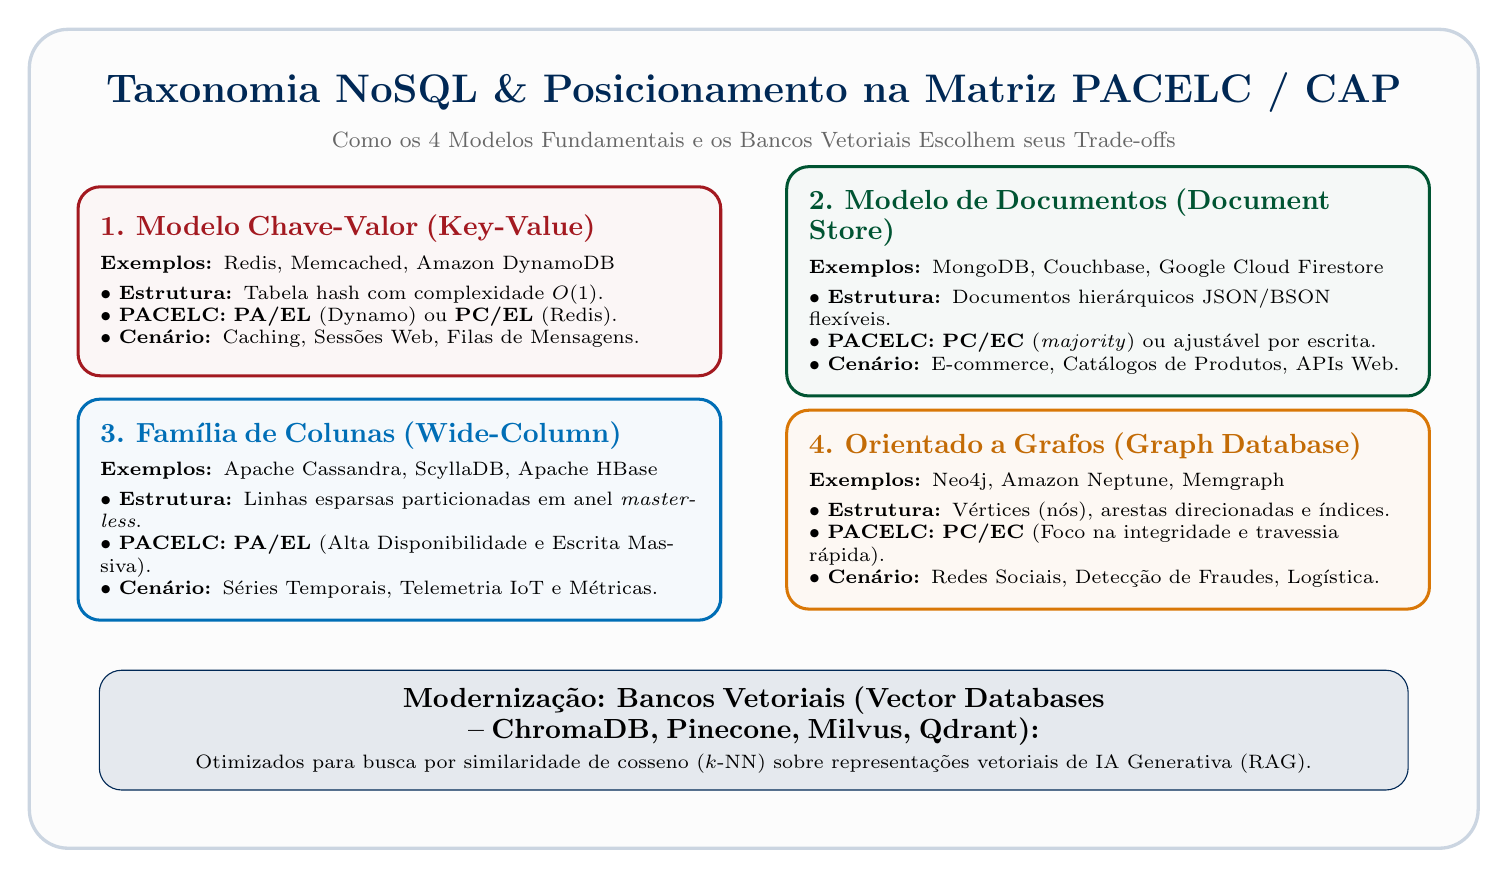
\begin{tikzpicture}[
    font=\sffamily,
    modelbox/.style={draw=BorderGray, rounded corners=8pt, fill=white, line width=1.1pt, align=left, inner sep=8pt, font=\scriptsize}
]

  % Painel Fundo Geral
  \node[draw=BorderGray, rounded corners=14pt, fill=gray!2, line width=1.2pt, minimum width=18.4cm, minimum height=10.4cm] (bg) at (0, 0) {};
  
  \node[font=\bfseries\Large, text=ScoutNavy] at (0, 4.4) {Taxonomia NoSQL \& Posicionamento na Matriz PACELC / CAP};
  \node[font=\footnotesize, text=gray!80!black] at (0, 3.8) {Como os 4 Modelos Fundamentais e os Bancos Vetoriais Escolhem seus Trade-offs};

  % =========================================================================
  % 1. CHAVE-VALOR (SUPERIOR ESQUERDO)
  % =========================================================================
  \node[modelbox, draw=ScoutRed, fill=ScoutRed!4, text width=7.6cm, minimum height=2.4cm] (m_kv) at (-4.5, 2.0) {
    \textbf{\color{ScoutRed}\normalsize 1. Modelo Chave-Valor (Key-Value)}\\[4pt]
    \textbf{Exemplos:} Redis, Memcached, Amazon DynamoDB\\[3pt]
    $\bullet$ \textbf{Estrutura:} Tabela hash com complexidade $O(1)$.\\
    $\bullet$ \textbf{PACELC:} \textbf{PA/EL} (Dynamo) ou \textbf{PC/EL} (Redis).\\
    $\bullet$ \textbf{Cenário:} Caching, Sessões Web, Filas de Mensagens.
  };

  % =========================================================================
  % 2. DOCUMENTOS (SUPERIOR DIREITO)
  % =========================================================================
  \node[modelbox, draw=ScoutGreen, fill=ScoutGreen!4, text width=7.6cm, minimum height=2.4cm] (m_doc) at (4.5, 2.0) {
    \textbf{\color{ScoutGreen}\normalsize 2. Modelo de Documentos (Document Store)}\\[4pt]
    \textbf{Exemplos:} MongoDB, Couchbase, Google Cloud Firestore\\[3pt]
    $\bullet$ \textbf{Estrutura:} Documentos hierárquicos JSON/BSON flexíveis.\\
    $\bullet$ \textbf{PACELC:} \textbf{PC/EC} (\textit{majority}) ou ajustável por escrita.\\
    $\bullet$ \textbf{Cenário:} E-commerce, Catálogos de Produtos, APIs Web.
  };

  % =========================================================================
  % 3. FAMÍLIA DE COLUNAS (INFERIOR ESQUERDO)
  % =========================================================================
  \node[modelbox, draw=ScoutBlue, fill=ScoutBlue!4, text width=7.6cm, minimum height=2.4cm] (m_col) at (-4.5, -0.9) {
    \textbf{\color{ScoutBlue}\normalsize 3. Família de Colunas (Wide-Column)}\\[4pt]
    \textbf{Exemplos:} Apache Cassandra, ScyllaDB, Apache HBase\\[3pt]
    $\bullet$ \textbf{Estrutura:} Linhas esparsas particionadas em anel \textit{masterless}.\\
    $\bullet$ \textbf{PACELC:} \textbf{PA/EL} (Alta Disponibilidade e Escrita Massiva).\\
    $\bullet$ \textbf{Cenário:} Séries Temporais, Telemetria IoT e Métricas.
  };

  % =========================================================================
  % 4. GRAFOS (INFERIOR DIREITO)
  % =========================================================================
  \node[modelbox, draw=ScoutAmber, fill=ScoutAmber!5, text width=7.6cm, minimum height=2.4cm] (m_graph) at (4.5, -0.9) {
    \textbf{\color{ScoutAmber!90!black}\normalsize 4. Orientado a Grafos (Graph Database)}\\[4pt]
    \textbf{Exemplos:} Neo4j, Amazon Neptune, Memgraph\\[3pt]
    $\bullet$ \textbf{Estrutura:} Vértices (nós), arestas direcionadas e índices.\\
    $\bullet$ \textbf{PACELC:} \textbf{PC/EC} (Foco na integridade e travessia rápida).\\
    $\bullet$ \textbf{Cenário:} Redes Sociais, Detecção de Fraudes, Logística.
  };

  % =========================================================================
  % FAIXA INFERIOR: BANCOS VETORIAIS (MODERNIZAÇÃO)
  % =========================================================================
  \node[draw=ScoutNavy, rounded corners=8pt, fill=ScoutNavy!10, font=\scriptsize, align=center, text width=16.2cm, inner sep=6pt] at (0, -3.7) {
    \textbf{\normalsize Modernização: Bancos Vetoriais (Vector Databases -- ChromaDB, Pinecone, Milvus, Qdrant):}\\[3pt]
    Otimizados para busca por similaridade de cosseno ($k$-NN) sobre representações vetoriais de IA Generativa (RAG).
  };

\end{tikzpicture}
\end{document}
